\documentclass{article}[12pt]
%% This is a template I've used for a lot of classes.
%% I think the set lengths actually came from a 350 homework assignment.
    \usepackage{textcomp}
    \usepackage{amsmath}
    \usepackage{amsfonts}
    \usepackage{amsthm}
    \usepackage{graphicx}
    \usepackage{setspace}
    \usepackage{gensymb}
    \usepackage{mathtools}
    \pdfpagebox5

    \setlength{\oddsidemargin}{0pt}
    \setlength{\evensidemargin}{0pt}
    \setlength{\textwidth}{6.5in}
    \setlength{\topmargin}{0in}
    \setlength{\textheight}{8.5in}
    \newcommand*\mean[1]{\bar{#1}}
    \newcommand*\pageline{\noindent\rule{\textwidth}{1pt}}
    \DeclarePairedDelimiter\hfloor{\lfloor\!\lfloor}{\rfloor\!\rfloor} % Credit goes to a Stack Exchange user named You.

% Template for homework answers!
%    \noindent\rule{\textwidth}{1pt}
%    \noindent \emph{()}
%    \[\boxed{}\]

\title{CSE 305, Principles of Database Systems \\ Assignment 1}
\author{Chris Morales\\Anthony Mulieri\\David Shank
\bigskip
% \\Collaborators: \\ Divjot Arora \\ Freeman Lou \\ Tony Mulieri \\ Rohith Rokkam \\ Bradley Wellman
}

\begin{document}
\doublespacing\maketitle

\newpage
\section*{Description}
The tool we used was ERD Plus, located at https://erdplus.com/\#/standalone.\\
Below, we explain some of the decisions we made:\\
Each user references a shopping cart, which contains a total price of the items within. The
taken\_items reference the shopping cart that they are in, and are removed from the quantity of the
item table. Once a user completes a purchase, a new empty shopping cart is created for the user, and
the old one is referenced by an entity in the purchase table.\\
We separated ‘address’ into it’s own table, so that processing it into a Java object would be
easier, allowing for more efficient conversion of the address into a string.\\
We did not make a distinction between merchants and buyers, encompassing both into the ‘user’ table.
We did not think that merchants should be the only ones eligible to sell items, nor should users
have to make a new account just to sell an item. All users can sell items, and all users can buy
items. Each item just has a reference to the user who is selling it.\\
We did not store the payment information for each user, although we may do this later depending on
how we feel.\\
Administrator is a table containing the user\_id of the user who is the administrator, separated into
a different table so that the administrators can have special permissions.\\
Each item will only have one category, although if this changes, we will update the implementation
by having the items have a set of predefined tags that reference the category.\\
\newpage
\section*{Diagrams}
Included are the final diagram and the inital paper prototype.
    \begin{figure}
        \centering
        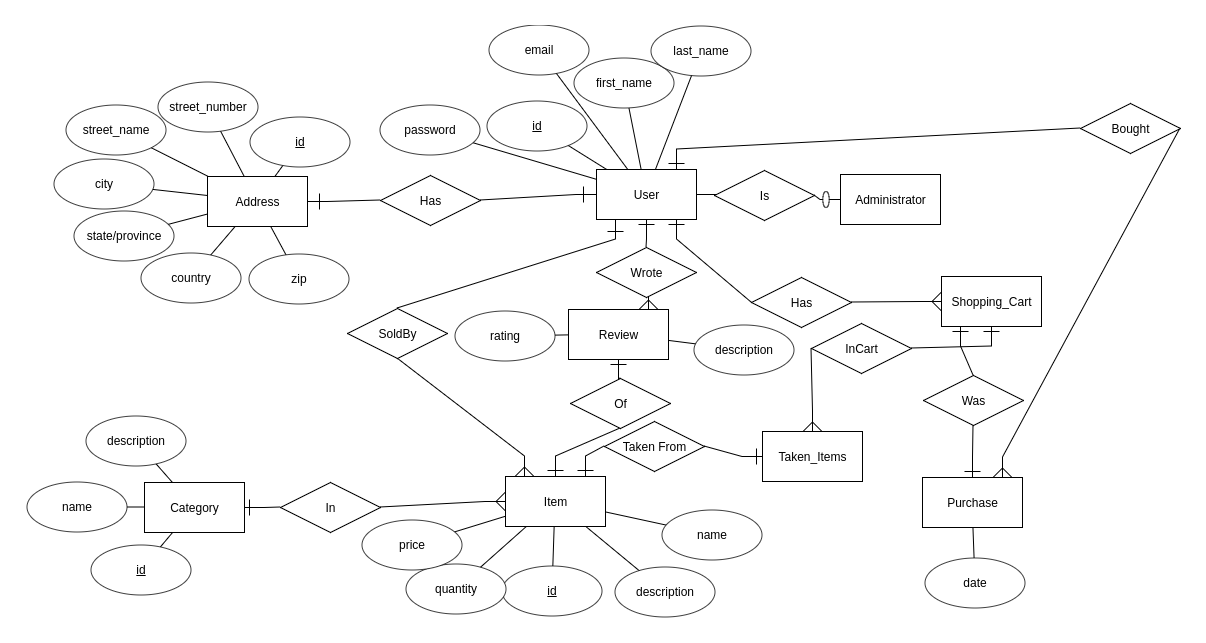
\includegraphics[width=\textwidth]{erdplus-diagram.png}
        \caption{Final ER Diagram}
    \end{figure}

    \begin{figure}
        \centering
        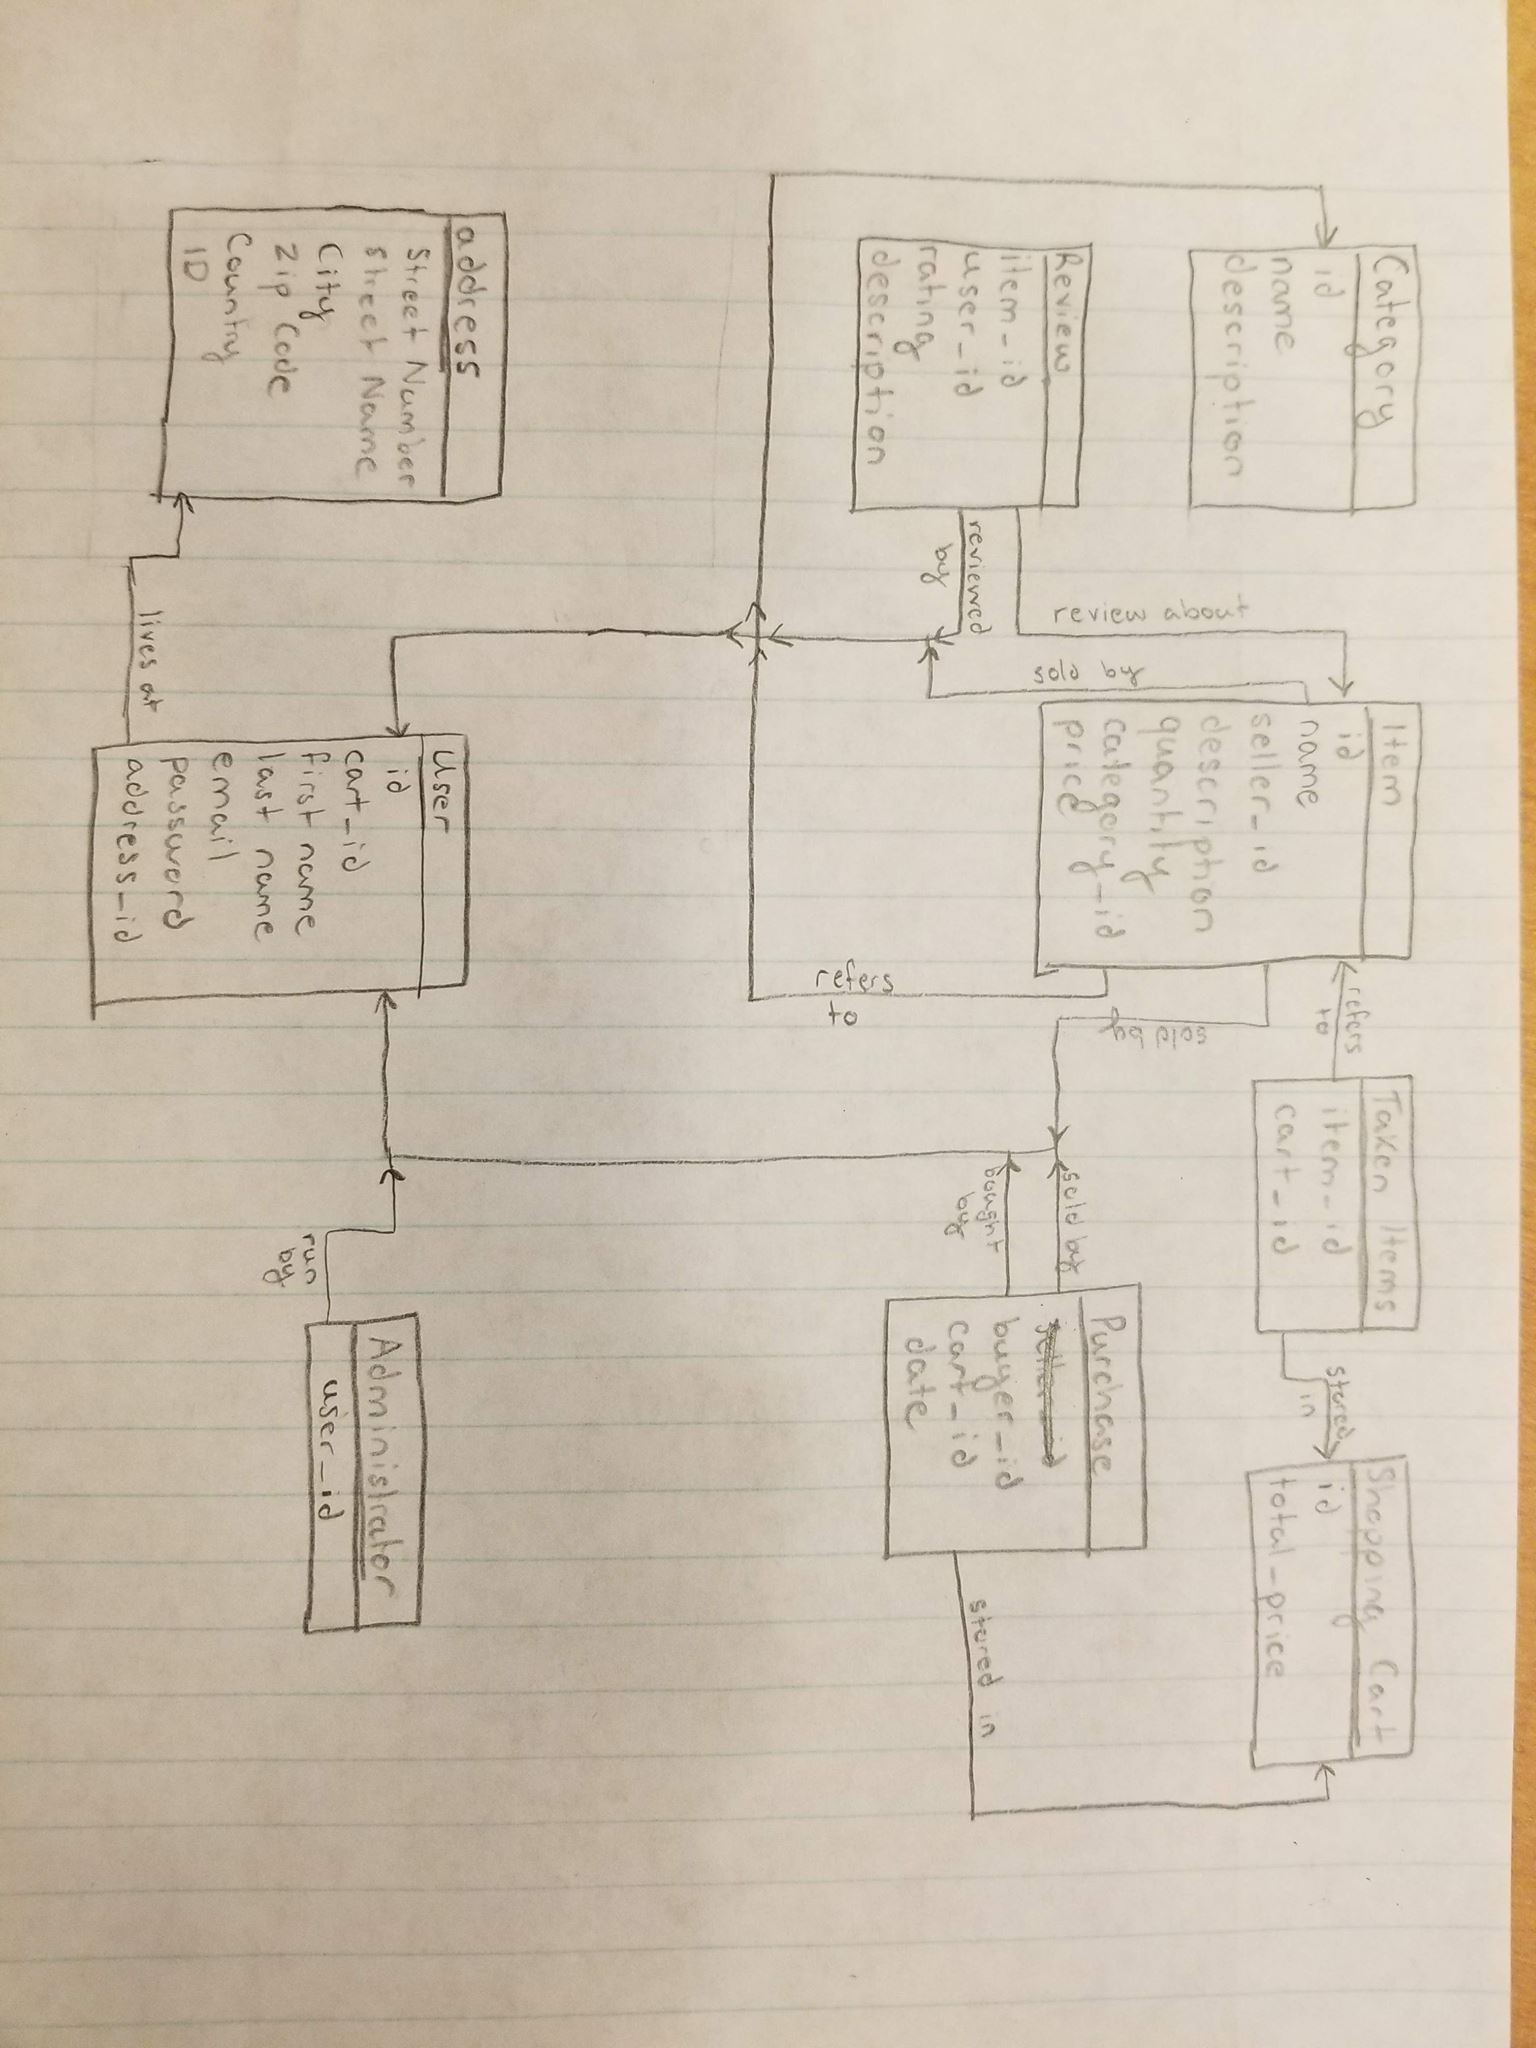
\includegraphics[angle=90,origin=c,width=\textwidth]{originaldiagram.jpg}
        \caption{Initial prototype}
    \end{figure}
\end{document}
